\chapter{基礎知識}

\section{ニュース番組のインデクシング}
ニュース音声のインデクシングは図\ref{fig:indexing}の手順で行われる。

\begin{figure}[H]
  \begin{center}
    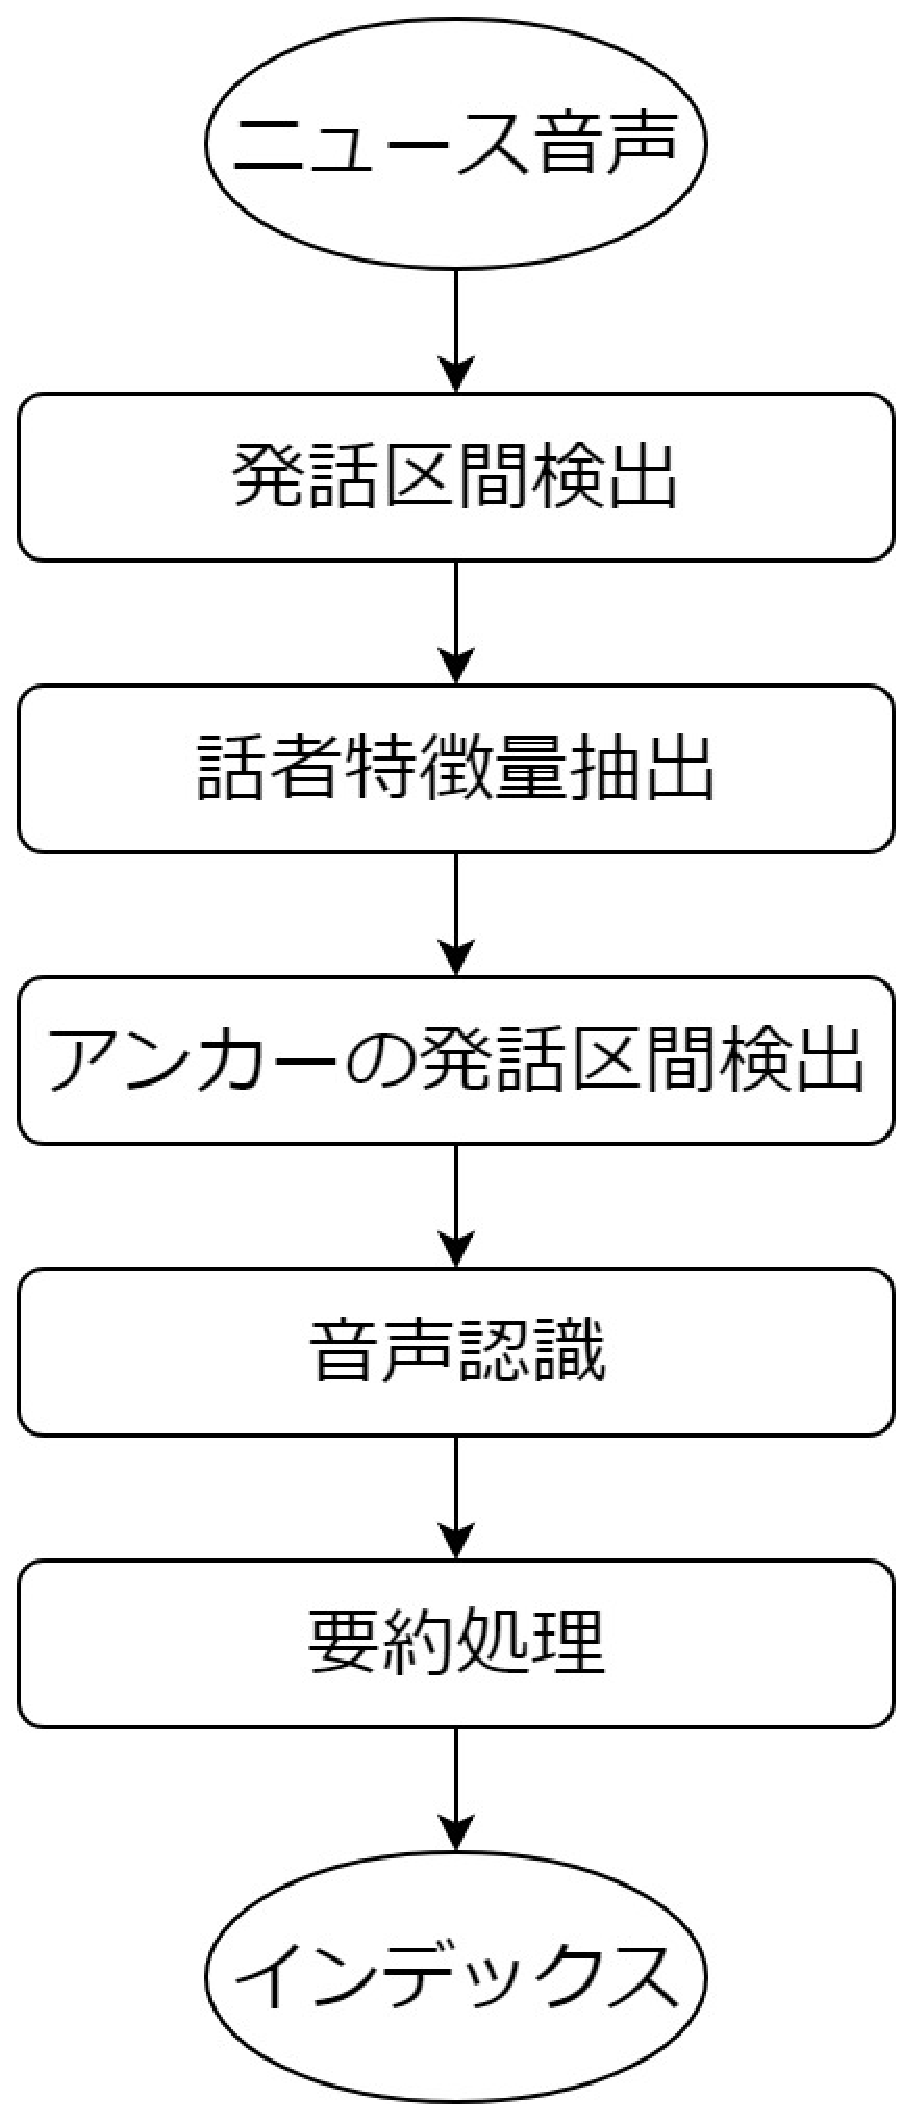
\includegraphics[scale=0.3]{./figure/indexing.eps}
  \end{center}
  \caption{インデクシングの手順 \label{fig:indexing}}
\end{figure}

入力であるニュース音声はどの区間で発話されているか未知であるため、まず音源分離によって発話区間検出を行う。次に検出した発話区間の中からアンカーの発話区間を検出するために、発話から話者特徴量を抽出し、発話をクラスタリングすることでアンカーの発話区間を検出する。検出されたアンカーの発話区間の音声認識を行い、認識結果の要約処理を行うことでインデックスが作成される。本稿では、ニュース音声の発話区間検出から音声認識までを行う。本稿で使用する技術について、本節以降で説明を行う。

\section{音源識別}
\label{section:devide_audio}
\renewcommand{\labelenumi}{(\arabic{enumi})}
音響データ(ニュース音声、会話音声等)の中にはさまざまな音源種別(声、音楽、雑音等)の音が混在している。音源識別とは、音響データ中に含まれる音源種別を自動的に識別することである。ここでの処理は、音響データのスペクトル解析を行い、音響特徴パラメータを求め、あらかじめ用意した各音源種別の音響特徴パラメータの分布と比較することで音源種別を識別する。\par
本研究では、ニュース番組の音声データに音響特徴パラメータを用いた音源識別\cite{shimae_9} を用い、音声データ中の音源種別を以下の4つに分類した。

\begin{enumerate}
\item 音声区間: アナウンサーやインタビューの声
\item 音楽区間: オープニングやエンディングなどの音楽、BGM
\item 背景雑音区間: 自動車走行音や鳥の泣き声
\item 無音区間: 音量が極めて小さい区間
\end{enumerate}\par

また、音源識別システムは音響データを各種別へ識別するための音響特徴パラメータの分布に混合ガウス分布を用いている。本研究では、混合数8のガウス分布を使用している。本研究の音響特徴パラメータを表2.2、各音源種別の識別性能F 値を表\ref{ad_F} に示す。ただし、表の評価値とは、音源種別間のデータ数を考慮するために、各音源種別のF 値に各音源種別の割合をかけ、合計したものである。\par

表2.2: 音源識別のための音響特徴パラメータ

\begin{table}[htb]
  \begin{center}
    \caption{音源識別システムのF値}
    \label{ad_F}
    \begin{tabular}{|c||c|} \hline
       & F値$[\%]$\\ \hline
      Speech & 94.84  \\ \hline
      Music & 83.32 \\ \hline
      Noise & 63.73  \\ \hline
      Pause & 77.43 \\ \hline
      評価値 & 87.19 \\ \hline
    \end{tabular}
  \end{center}
\end{table}



以下に、音源識別のためのスペクトル解析と音響特徴パラメータについて説明する。\par


\subsection{スペクトル解析}
音響データのスペクトル解析の手法として最も一般的に利用されている方法は、短時間フーリエスペクトル分析がある。この方法は、音響データから連続する数10ms 程度の時間長の信号区間を切り出し、切り出された信号が定常性(一定周期で繰り返す)と仮定して、スペクトル解析を行う。\par
スペクトル解析の流れは以下の通りである。

\begin{enumerate}
\item フレーム化処理:与えられた信号$s(n)$ に長さ$N$ の分析窓を掛けることで以下のような信号系列$s_\omega(m; l)$を取り出す。
\begin{equation}
S_w(m;l)=\sum_{m=0}^{N-1}\omega(m)s(l+m)\qquad(l=0,T,2T,\cdots)
\end{equation}

ここで、添え字$l$は信号の切り出し位置に対応している。すなわち、$l$を一定間隔$T$で増加させることで定常とみなされる長さ$N$の信号系列$s_\omega(n)\quad (n=0,1,\cdots,N-1)$が間隔$T$で得られる。この処理をフレーム化処理と呼び、$N$をフレーム長、$T$をフレーム間隔と呼ぶ。

\item 窓関数をかける:ある有限区間以外で0となる関数であり、フレーム化されたデータに対して重みをつける関数である。フレーム化処理を行う場合、離散的なデータの繋ぎ目においての信号の急激な変化の影響を和らげるため、原則として窓関数をかけなければならない。代表的なものとして音声信号だけに有効なハニング窓と、音声信号以外にも様々な信号にも有効なハミング窓がある。

\begin{equation}
\label{da1}
ハニング窓:\omega(n)=0.5-0.5\cos(\frac{2\pi n}{N-1})\qquad(n=0,1,\cdots,N-1)
\end{equation}

\begin{equation}
\label{da2}
ハミング窓:\omega(n)=0.54-0.54\cos(\frac{2\pi n}{N-1})\qquad(n=0,1,\cdots,N-1)
\end{equation}

\item スペクトル分析(離散時間フーリエ変換、高速フーリエ変換):フレーム化処理によって得られた信号系列の短時間フーリエスペクトルは、離散時間フーリエ変換により以下の式で与えられる。
\begin{equation}
S(n)=\sum s_\omega(n)e^{-j2\pi \frac{nk}{N}} \qquad (k=0,1,\cdots,N-1)
\end{equation}

離散フーリエ変換(DFT) は、離散的なデータをフーリエ変換する際に、通常のフーリエ変換の無限区間積分を有限の和で書き換えたもので、時間領域、周波数領域ともに離散化されたフーリエ変換のことであり、時間領域の表現を周波数領域における表現に変換する。また、逆に周波数領域の表現を時間領域の表現に変換する、つまり元の音響データに戻す変換を離散フーリエ逆変換(IDFT) と呼び以下の式で与えられる。

\begin{equation}
S(n)=\frac{1}{N}\sum S(k)e^{j2\pi \frac{nk}{N}} \qquad (k=0,1,\cdots,N-1)
\end{equation}

実際の信号処理過程では、離散的フーリエ変換(DFT) をその高速算法である高速フーリエ変換(FFT) を用いて実行し、当該音声区間のスペクトル表現とすることが一般的である。高速フーリエ変換は式(\ref{da1})、(\ref{da2}) の$N$ が$2^n$ 個であるとき、その処理を高速にできる性質がある。フーリエ変換の式には、

\begin{equation}
S\prime(n)=S(e^{j\frac{2\pi}{n}k})=\sum s_\omega(n)e^{-j2\pi \frac{2\pi}{N}kn} \qquad (k=0,1,\cdots,N-1)
\end{equation}

なる複素系列$S\prime(k)$が音声スペクトル表現として最も一般的に用いられる。

\item パワースペクトルの算出:音響信号の特徴は主として、調音フィルタの振幅伝達特性に含まれる。したがって、音響信号の振幅スペクトル$|S^\prime(k)|$、あるいはその2 乗のパワースペクトル$|S^\prime(k)|^2$、対数スペクトル$10\log|S^\prime(k)|^2$が注目すべきスペクトル表現になる。このスペクトルをグラフにすることで、音響データに含まれている周波数成分を解析することができる。音響データに含まれている周波数成分の上限はサンプリング定理により、サンプリング周波数の半分なので、高速フーリエ変換における周波数成分が意味のあるスペクトルとして扱われるのは0 から$\pi$までのスペクトルである。また、音響信号の離散パワースペクトル系列は、離散スペクトル系列から式(\ref{da3}) で表される。

\begin{equation}
\label{da3}
|S^\prime(k)|^2=\frac{1}{N}[\operatorname{Re}\left\{S^\prime(k)\right\}^2+\operatorname{Im}\left\{S^\prime(k)\right\}^2]
\end{equation}

この2 乗値のパワースペクトル$|S^\prime(k)|^2$を特徴量として扱っている。音響信号に高速フーリエ変換を施すと、時間表現(縦軸:パワー、横軸:時間) から周波数表現(縦軸:振幅、横軸:周波数) へと変換できる。しかし、実際には縦軸を周波数、横軸を時間としたグラフがよく使用されており、このようなグラフをスペクトルグラムという。スペクトルグラムは音声を視覚化したものであり、声紋とも呼ばれる。

\end{enumerate}\par
\subsection{音響特徴パラメータ}
本研究で使用する7つの音響特徴パラメータについて述べる\cite{shimae_10}

\begin{enumerate}
\item スペクトルの変化\par
動的特徴量を連続するスペクトルのフレーム間の変化量として取り出す。音響信号のスペクトル分析した連続するフレームにおいて、あるフレームとその一定時間後のフレームとのパワースペクトルの差分によりスペクトルの変化量を得て、そのスペクトルの差分を一定時間足し合わせたものとしている。スペクトルの変化量によって比較する利点は、音声の識別に有利であり音声に比べて背景雑音のほうがスペクトルの変化量が大きく、無音のほうがスペクトルの変化量が小さいということである。

\item スペクトルの傾き\par
あらかじめ人手により作成したラベルにより音響データの各区間を各種別(音声、音楽、背景雑音、無音)に振り分け、それぞれに対してスペクトル分析を行い、パワースペクトルを取り出し、各種別内において集められたパワースペクトルの分布を求めることで各種別において傾き値を得る。この傾き値を基に、与えられた音響ファイルから次々に得るパワースペクトルと各種別の学習データとの特徴パラメータの分布の類似度を比較する。この最小単純形は、パワースペクトルにおける一次回帰直線の傾きを比べることと同じである。傾きによって比較する利点は、有色系の音のほうが白色雑音よりも傾きが大きいので、音声と音楽と無音の識別に有利である。

\item 白色雑音との近さ\par
パワースペクトルより一次回帰直線からスペクトル波形の切片を求めることで入力信号の白色性の度合を計測する。この白色雑音との近さによって比較する利点は、背景雑音のような定常的に混入した雑音は白色性が高いので、これらの識別ができるこということである。

\item ピッチ\par
有声音源の繰り返し周期、いわゆるピッチ(基本周波数)の変化を調べることで、音源の変化を知ることができ、音源の特定のパラメータである。周波数分析によりピッチを求め、学習データと比べることで音源の特定に用いる。

\item パワー\par
時間領域の分析だが、音響信号のような非定常的な信号に対して、変化していく信号の大きさにうまく追随するような比較的短い区間に音響データを区切り、その区間の信号$xl(n)$に対してエネルギー$E(l)$ を定義する\cite{shimae_11}。
\begin{equation}
E(l)=\sum_{n=0}^{N-1}\left\{x_l(n)\right\}^2
\end{equation}
ここでは、整数$N$ は窓の中に含まれる音響信号の数である。\par
利点としては、測定が簡単であり、音声認識における有色系の音の区間の抽出にもよく用いられることから、有音と無音の区別に有利である。

\item 中心周波数\par
抽出したパワースペクトルにおいて、無音の場合は右下がりに傾斜しているが、有音の場合は傾斜の途中で膨らみまたは突起が発生する。その突起がもっとも大きく発生している周波数帯の中心部分の周波数を中心周波数として定義している。これは有音と無音の識別に効果がある。

\item 中心周波数のバンド幅\par
中心周波数を含む膨らみ、あるいは突起の始まりと終わりによる周波数帯の長さをバンド幅として定義する。音声は一定の周波数を含むことが多いためそのバンド幅はある程度の大きさになることが考えられるが、雑音はあまり多くの周波数を含まないものから白色性が高く幅広い周波数を含むものまで様々であり、その違いから音声と雑音の特定に有効である。
\end{enumerate}\par


\section{i-vectorの概要}
\subsection{UBMに対するBaum-Welch統計量}
すすす
\subsection{全因子$w$の確率分布とi-vectorの抽出}
あ
\subsection{因子分析モデルパラメータの推定}
あ
\subsection{コサイン類似度}
あ


\section{音声認識}
\subsection{音声認識システムの流れ}

\subsection{単語辞書と言語モデル}
\textbf{\underline{単語辞書}}\par
a
\par\textbf{\underline{言語モデル}}\par
\par\textbf{\underline{Nグラムモデル}}\par

\subsection{音響モデル}
\par\textbf{\underline{MFCC}}\par
\par\textbf{\underline{隠れマルコフモデル(HMM)}}\par
\par\textbf{\underline{調音結合}}\par

\subsection{DNNの概要}

